\documentclass[t]{beamer}
\usetheme[deutsch]{KIT}
\setbeamercovered{transparent}
\setbeamertemplate{navigation symbols}{}

\KITfoot{Tutoriumsmaterial von Alexander Kwiatkowski, Michael Vollmer und Matthias Holoch \hspace{2.5cm} Basierend auf den Folien von Simon Stroh und Moritz v. Looz}
\usepackage[utf8]{inputenc}
\usepackage{amsmath}
\usepackage{ifthen}
\usepackage{amssymb}
\usepackage{tikz}
\usepackage{ngerman}
\usepackage[normalem]{ulem}
\usetikzlibrary{automata}
\usenavigationsymbols


\title{Theoretische Grundlagen der Informatik}
\subtitle{Tutorium}
\author{Alexander Kwiatkowski, Michael Vollmer und Matthias Holoch}

\institute[IKS]{Institut für Kryptographie und Sicherheit}

\TitleImage[height=\titleimageht]{images/tmaschine.png}

\newcommand{\N}{\ensuremath{\mathbb{N}}}
\newcommand{\M}{\ensuremath{\mathcal{M}}}
\newcommand{\classP}{\ensuremath{\mathcal{P}}}
\newcommand{\classNP}{\ensuremath{\mathcal{NP}}}
\newcommand{\co}{\ensuremath{\mathsf{co\text{-}}}}
\newcommand{\pot}{\ensuremath{\mathcal{P}}}
\newcommand{\abs}[1]{\ensuremath{\left\vert #1 \right\vert}}
\newcommand{\menge}[2]{\ensuremath{\left\lbrace #1 \,\middle\vert\, #2 \right\rbrace}}
\newcommand{\ducttape}[1]{\vspace{#1}}
\newcommand{\neglit}[1]{\overline{#1\vphantom{x^a}}}
\newcommand{\recipe}{\raisebox{-.3cm}{
\includegraphics[scale=.15]{images/chefs-cap.png}}\hspace{0.2cm}}
\newcommand{\opt}[1]{\ensuremath{\text{OPT}(#1)}}
\newcommand{\A}[1]{\ensuremath{\mathcal{A}(#1)}}
\renewcommand{\O}[1]{\ensuremath{\mathcal{O}(#1)}}
\newcommand{\msout}[1]{\text{\sout{\ensuremath{#1}}}}

\newcommand{\invincible}{\setbeamercovered{invisible}} %  "Yesss! I am invincible!!" (Boris Grishenko)
\newcommand{\vincible}{\setbeamercovered{transparent}}
\renewcommand{\solution}[1]{\invincible \pause #1 \vincible}
\newcommand{\micropause}{\\[8pt]}

% \@ifundefined{tikzset}{}{\tikzset{initial text=}} % Text "start" bei Startknoten unterdrücken
\tikzstyle{every node}=[thick]
\tikzstyle{every line}=[thick]

\newcommand{\tutnr}[1]{
  \subtitle{Tutorium #1}
	\begin{frame}
		\maketitle
	\end{frame}
}

\newcommand{\uebnr}[1]{
  \subtitle{Anmerkungen zum #1. Übungsblatt}
	\begin{frame}
		\maketitle
	\end{frame}
}

\begin{document}

\newcommand{\start}[3]
{
  \draw (#1*2,#2*2) node{$#3$};
  \draw (#1*2,#2*2) circle(0.4cm);
  \draw [->] (#1*2-0.9,#2) -- (#1*2-0.4,#2);
}
\newcommand{\final}[3]
{
  \draw (#1*2,#2*2) node{$#3$};
  \draw (#1*2,#2*2) circle(0.4cm);
  \draw (#1*2,#2*2) circle(0.32cm);
}
\newcommand{\startfinal}[3]
{
  \draw (#1*2,#2*2) node{$#3$};
  \draw (#1*2,#2*2) circle(0.4cm);
  \draw (#1*2,#2*2) circle(0.32cm);
  \draw [->] (#1*2-0.9,#2) -- (#1*2-0.4,#2);
}
\newcommand{\state}[3]
{
  \draw (#1*2,#2*2) node{$#3$};
  \draw (#1*2,#2*2) circle(0.4cm);
}
\newcommand{\tol}[4]
{
  \draw (#1+#3,#2*2) node[above]{$#4$};
  \draw [->] (#1*2-0.4,#2*2) -- (#3*2+0.4,#2*2);
}
\newcommand{\tor}[4]
{
  \draw (#1+#3,#2*2) node[above]{$#4$};
  \draw [->] (#1*2+0.4,#2*2) -- (#3*2-0.4,#2*2);
}
\newcommand{\tot}[4]
{
  \draw (#1*2,#2+#3) node[right]{$#4$};
  \draw [->] (#1*2,#2*2+0.4) -- (#1*2,#3*2-0.4);
}
\newcommand{\tob}[4]
{
  \draw (#1*2,#2+#3) node[right]{$#4$};
  \draw [->] (#1*2,#2*2-0.4) -- (#1*2,#3*2+0.4);
}
\newcommand{\totl}[5]
{
  \draw (#1+#3,#2+#4) node[above right]{$#5$};
  \draw [->] (#1*2-0.283,#2*2+0.283) -- (#3*2+0.283,#4*2-0.283);
}
\newcommand{\totr}[5]
{
  \draw (#1+#3,#2+#4) node[above left]{$#5$};
  \draw [->] (#1*2+0.283,#2*2+0.283) -- (#3*2-0.283,#4*2-0.283);
}
\newcommand{\tobl}[5]
{
  \draw (#1+#3,#2+#4) node[below right]{$#5$};
  \draw [->] (#1*2-0.283,#2*2-0.283) -- (#3*2+0.283,#4*2+0.283);
}
\newcommand{\tobr}[5]
{
  \draw (#1+#3,#2+#4) node[below left]{$#5$};
  \draw [->] (#1*2+0.283,#2*2-0.283) -- (#3*2-0.283,#4*2+0.283);
}
\newcommand{\rloopl}[3]
{
  \draw (#1*2-1,#2*2) node[left]{$#3$};
  \draw [->] (#1*2-0.35,#2*2-0.2) arc (-30:-320:0.32cm);
}
\newcommand{\rloopr}[3]
{
  \draw (#1*2+1,#2*2) node[right]{$#3$};
  \draw [->] (#1*2+0.35,#2*2+0.2) arc (150:-140:0.32cm);
}
\newcommand{\rloopt}[3]
{
  \draw (#1*2,#2*2+1) node[above]{$#3$};
  \draw [->] (#1*2-0.2,#2*2+0.35) arc (240:-50:0.32cm);
}
\newcommand{\rloopb}[3]
{
  \draw (#1*2,#2*2-1) node[below]{$#3$};
  \draw [->] (#1*2+0.2,#2*2-0.35) arc (60:-230:0.32cm);
}
\newcommand{\lloopl}[3]
{
  \draw (#1*2-1,#2*2) node[left]{$#3$};
  \draw [->] (#1*2-0.35,#2*2+0.2) arc (30:320:0.32cm);
}
\newcommand{\lloopr}[3]
{
  \draw (#1*2+1,#2*2) node[right]{$#3$};
  \draw [->] (#1*2+0.35,#2*2-0.2) arc (-150:140:0.32cm);
}
\newcommand{\lloopt}[3]
{
  \draw (#1*2,#2*2+1) node[above]{$#3$};
  \draw [->] (#1*2+0.2,#2*2+0.35) arc (-60:230:0.32cm);
}
\newcommand{\lloopb}[3]
{
  \draw (#1*2,#2*2-1) node[below]{$#3$};
  \draw [->] (#1*2-0.2,#2*2-0.35) arc (-240:50:0.32cm);
}
\include{amsmath}

\tutnr{12}

\section{Begriffe der Informationstheorie}
%Erklären: (gedächtnislose) Quelle, Entropie, Informationsgehalt, Ordnung von Zeichenketten
\subsection{Erklärung}
\subsection{Aufgabe B11 A1}
\begin{frame}
	\frametitle{Aufgabe B11 A1}
	\begin{enumerate}
		\item Wie gro"s sind der Informationsgehalt und die Entropie, wenn eine Quelle mit
		dem Alphabet $\{0,1\}$ nur aus dem Zeichen $0$ bestehende Folgen sendet?
		\item An einer Quelle mit $n$ Zeichen tritt jedes Zeichen gleichverteilt auf. Wie
		gro"s sind der Informationsgehalt und die Entropie eines einzelnen Zeichens?
		\item Berechnen Sie die Entropie des Wurfes eines idealen W"urfels mit 8 Seiten,
		dessen Wahrscheinlichkeit f"ur jede Seite $p = \frac{1}{8}$ ist!
		\item Was ist der Unterschied zwischen den beiden Folgen, die aus verschiedenen
		ged"achtnislosen Quellen mit der gleichen Wahrscheinlichkeit f"ur $0$ und $1$
		gesendet werden, wenn man sie unter dem Aspekt Entropie und Ordnung betrachtet?
		\begin{enumerate}
			\item ...10101010101010101010...
			\item ...01101100110111000010...
		\end{enumerate}
	\end{enumerate}
\end{frame}

\section{Mehr Begriffe der Informationstheorie}
%Erklären: Empfänger, Kanäle, Verbundentropie, Irrelevanz, Äquivokation, Transinformation, Fehlinformation(="inverse Äquivokation"=Irrelevanz?), Totalinformation (=Verbundentropie?)
\subsection{Erklärung}
\subsection{Aufgabe B11 A2}
\begin{frame}
	\frametitle{Aufgabe B11 A2}
	\only<1>{
	Studieren Sie den Fall eines asymmetrischen bin"aren Kanals mit Quelle $X$ und
	Empf"anger $Y$. Die "Ubertragungswahrscheinlichkeiten $P(Y|X)$ seien durch das
	folgende Diagramm gegeben:
	}
	\vspace{-0.6cm}
		\begin{center}
			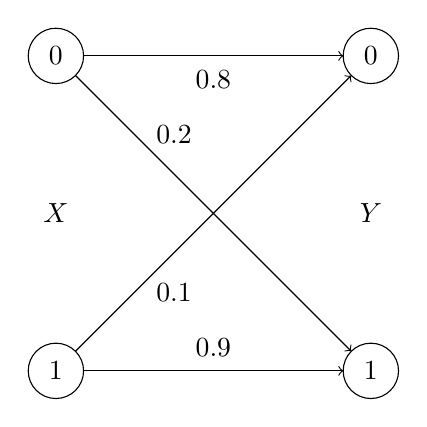
\begin{tikzpicture}
			\draw (0,0) circle (10pt);
			\draw (0,0) node {$1$};
			\draw (0,2) node {$X$};
			\draw (0,4) circle (10pt);
			\draw (0,4) node {$0$};
			\draw (4,0) circle (10pt);
			\draw (4,0) node {$1$};
			\draw (4,2) node {$Y$};
			\draw (4,4) circle (10pt);
			\draw (4,4) node {$0$};
			\draw [->] (0.35,0) -- (3.65,0);
			\draw (2,0.3) node {$0.9$};
			\draw [->] (0.35,4) -- (3.65,4);
			\draw (2,3.7) node {$0.8$};
			\draw [->] (0.25,0.25) -- (3.75,3.75);
			\draw (1.5,1) node {$0.1$};
			\draw [->] (0.25,3.75) -- (3.75,0.25);
			\draw (1.5,3) node {$0.2$};
			\end{tikzpicture}
		\end{center}
		\only<2,3>{
	\begin{enumerate}
		\only<2>{
		\item Wie gro"s ist die Wahrscheinlichkeit daf"ur, dass die Bitkette ``$1100$'' als
		``$1001$'' "ubertragen wird?
		\item Wenn die Entropie der Quelle $H(X) = 1 \; \mbox{bit}$ ist, wie gro"s ist dann
		$H(Y)$?
		\item Wie gro"s muss $H(X)$ sein, damit $H(Y) = 1 \; \mbox{bit}$ gilt?
		}
		\only<3>{
		\item Wie gro"s ist die Verbundentropie $H(X,Y)$ des "Ubertragungssystems? Gehen Sie
		ab dieser Teilaufgabe von der Situation der 2. Teilaufgabe aus!
		\item Wie gro"s ist die sog. Irrelevanz $H(Y|X)$? Und wie gro"s ist die sog.
		"Aquivokation $H(X|Y)$?
		\item Wie gro"s ist schlie"slich die Transinformation $I(X;Y)$?	
	}
	\end{enumerate}
	}
\end{frame}
\subsection{Aufgabe B11 A4}
\begin{frame}
	\frametitle{Aufgabe B11 A4}
	Gegeben sei eine ged"achtnislose Quelle $Q$, die mit Wahrscheinlichkeit $p_0 =
	\frac{1}{4}$ eine $0$ und mit Wahrscheinlichkeit $p_1 = \frac{3}{4}$ eine $1$ sendet.
	Gegeben sei zudem ein Empf"anger $R$, der die Zeichen von $Q$ zu empfangen versucht.
	Dieser Empf"anger empf"angt eine $0$ immer richtig. Sendet die Quelle $Q$ jedoch
	eine $1$, so empf"angt $R$ mit Wahrscheinlichkeit $\frac{1}{2}$ eine $1$ und mit
	Wahrscheinlichkeit $\frac{1}{2}$ eine $0$.
	\begin{enumerate}
		\item Berechnen Sie die Information $I(0)$ und $I(1)$ bez"uglich der Quelle $Q$!
		\item Berechnen Sie die Entropie der Quelle $Q$!
		\item Die Quelle $Q$ sendet die Zeichenfolge $0110$. Wie hoch ist der
		Informationsgehalt dieser Zeichenfolge?
		\item Berechnen Sie die Totalinformation $H(Q,R)$, die Fehlinformation $H(R|Q)$,
		die "Aquivokation $H(Q|R)$ und die Transinformation $I(Q;R)$!
	\end{enumerate}
\end{frame}

\section{Huffman-Codierung}
\subsection{Erklärung}
\subsection{Aufgabe B11 A3}
\begin{frame}
	\frametitle{Aufgabe B11 A3}
	Gegeben sei eine Quelle mit Alphabet $\{A,B,C,D\}$ und mit den folgenden
	Wahrscheinlichkeiten:\\
	$P(A)=\frac{1}{2}, P(B)=\frac{1}{4}, P(C)=\frac{1}{8}, P(D)=\frac{1}{8}$
	\begin{itemize}
	\only<1>{
		\item Berechnen Sie die Entropie der Quelle!
		\item Erstellen Sie eine entsprechende Huffman-Codierung!
		\item Was ist die mittlere Codewortl"ange? Gibt es einen Zusammenhang zur Entropie?
		}
		\only<2>{
		\item Gegeben sei der folgende Huffman-Baum:
		\begin{center}
			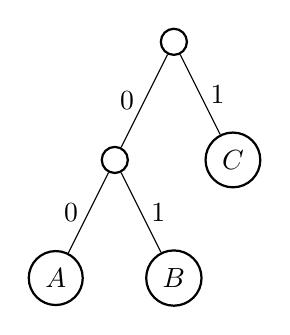
\begin{tikzpicture}
				\node[circle,draw]{}
				child{
				  node[circle,draw]{}
				  child{
				    node[circle,draw]{$A$}
				    edge from parent
				    node[left]{\textbf{$0$}}
				  }
				  child{
				    node[circle,draw]{$B$}
				    edge from parent
				    node[right]{\textbf{$1$}}
				  }
				  edge from parent
				  node[left]{\textbf{$0$}}
				}
				child{
				  node[circle,draw]{$C$}
				  edge from parent
				  node[right]{\textbf{$1$}}
				};
			\end{tikzpicture}
		\end{center}
		Dekodieren Sie $011011101100101011$! Ist der Huffman-Code geeignet?
		}
	\end{itemize}
\end{frame}

\section{Schluss}
\subsection{Schluss}
\begin{frame}
\frametitle{Bis zum nächsten Mal!}
%TODO change the comic
	\center{Kolmogorov Directions}
\begin{center}
	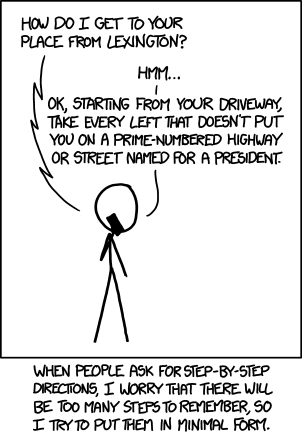
\includegraphics[height=0.85\textheight]{images/kolmogorov_directions.png}
\end{center}
\end{frame}

\frame{
  \frametitle{Lizenzen}
  \center
  
\includegraphics[width=2em]{images/by}
  
\includegraphics[width=2em]{images/cc}
  
\includegraphics[width=2em]{images/sa}
  \\
  {\tiny

Dieses Werk ist unter einem ``Creative Commons Namensnennung-Weitergabe unter gleichen Bedingungen 3.0 Deutschland``-Lizenzvertrag lizenziert. Um eine Kopie der Lizenz zu erhalten, gehen Sie bitte zu \href{http://creativecommons.org/licenses/by-sa/3.0/de/}{http://creativecommons.org/licenses/by-sa/3.0/de/} oder schreiben Sie an Creative Commons, 171 Second Street, Suite 300, San Francisco, California 94105, USA.\\
  \vspace{1cm}
  Davon ausgenommen sind das Titelbild, welches aus der März-April 2002 Ausgabe von American Scientist erschienen ist und ohne Erlaubnis verwendet wird, sowie das KIT Beamer Theme. Hierfür gelten die Bestimmungen der jeweiligen Urheber.
  \vspace{1cm}
  \\ 
  }
  %Habe hier die Reihenfolge etwas umgestellt, weil die Formatierung bei mir komisch aussah. 
  %Wenn es bei dir anders ist, kannst du es auch wieder zurückändern, dann haben wir unterschiedliche Kompilieroptionen
}

\end{document}